\clearpage
\section{Umsetzung}
Bei der Konzeptionierung und Entwicklung der Android App wurde Wert darauf gelegt, dass Programmlogik, Benutzeroberfläche, Exportfunktion und Datenbankanbindung soweit als möglich voneinander getrennt sind. Entsprechend sind diese Themen hier auch unabhängig voneinander beschrieben.

\subsection{Programmlogik / Backend}
\label{subsec:programmlogikbackend}
Das Backend unserer Android Applikation besteht aus den beiden Klassen Track und Waypoint. 

\begin{figure}[h]
  \centering
  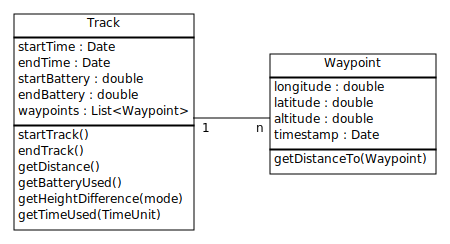
\includegraphics[width=0.8\textwidth]{images/classdiag_backend.pdf}
  \caption[Klassendiagramm Backend]{Klassendiagramm Backend}
  \label{fig:classdiag_backend}
\end{figure}

Im Klassendiagramm (Abbildung \ref{fig:classdiag_backend}) ist ersichtlich, dass ein Track primär aus einer Menge von Waypoints besteht. Zusätzlich werden Informationen zu Start- und Endzeit und Akkuzustand bei Start beziehungsweise Ende des Tracks mitgeführt. Die Waypoints bestehn aus den Koordinaten (Breiten- und Längengraden), der Höhe (Höhe über dem Geoiden) und einem Timestamp.

Der Track besitzt öffentliche Methoden zum Berechnen des Akkuverbrauchs, der Distanz, der Höhendifferenz und der Verbrauchten Zeit. Folgend wird kurz aufgezeigt wie die Funktionsweise dieser Methoden ist.

\begin{itemize}
\item \lstinline$getBatteryUsed()$ : $batteryUsed = startBattery-endBattery$ 
\item \lstinline$getDistance()$ : Siehe Kapitel \ref{subsec:distance}
\item \lstinline$getHeightDifference(mode)$ : Siehe Kapitel \ref{subsec:heightdifference}
\item \lstinline$getTimeUsed(TimeUnit)$ :
\begin{itemize}
	\item $timeUsedMs = endTime-startTime$
	\item $timeUsedS = \frac{endTime-startTime}{1000}$
	\item $timeUsedM = \frac{endTime-startTime}{1000*60}$
	\item $timeUsedH = \frac{endTime-startTime}{1000*60*60}$
	\item $timeUsedD = \frac{endTime-startTime}{1000*60*60*24}$
\end{itemize}
\end{itemize}

Weiter gibt es in der Klasse Track die beiden Methoden \lstinline$startTrack()$ und \lstinline$endTrack$, welche das Tracking an sich steuern. In der Methode \lstinline$startTrack$ (Listing \ref{lst:starttrack}) werden zuerst die beiden Einstellungen mithilfe des Android \lstinline$PreferenceManager$ ausgelesen. Als nächstes wird die StartZeit und der Batteriezustand beim Starten des Tracks festgehalten. Zum Schluss wird auf den \lstinline$LocationManager$ mithilfe des per Parameter übergebenen Contexts zugegriffen. Diesem \lstinline$LocationManager$ wird dann ein neuer \lstinline$LocationListener$ angehängt.

Beim Anhängen des \lstinline$LocationListener$s werden folgende Paramter mitgegeben: 
\begin{itemize}
	\item provider: Der Verwendete Provider für die Location Updates (in unserem Falle GPS)
	\item timeInterval: Das Zeitinterval. Wie oft soll der LocationListener angestossen werden?
	\item minDistance: Die minimale Distanz zwischen der aktuellen Location und der letzten. Wenn nach Ablauf des Zeitintervals diese Distanz nicht überschritten ist, wird der LocationListener nicht angestossen. \cite{locationmanager}
\end{itemize}

\begin{lstlisting}[caption={startTrack Methode}, label={lst:starttrack}]
private LocationListener = new LocationListener() {
	public void onLocationChanged(Location location) {
		// Called when a new location is found by the network location provider.
		trackLocation(location);
	}
}

public void startTrack(Context context) {
	//Read Settings
	SharedPreferences sharedPref = PreferenceManager.getDefaultSharedPreferences(context);
	long minDistance = Long.parseLong(sharedPref.getString("min_dist_between_tp", "10"));
	long timeInterval = Long.parseLong(sharedPref.getString("max_time_between_tp", "10000"));
	
	//set meta infos
	startTimestamp = new Date();
	startBatteryPercentage = getBatteryStatus(context);

	// Acquire a reference to the system Location Manager
	LocationManager locationManager = (LocationManager) context.getSystemService(Context.LOCATION_SERVICE);

	// Register the listener with the Location Manager to receive location updates
	locationManager.requestLocationUpdates(LocationManager.GPS_PROVIDER, timeInterval, minDistance, locationListener);
}
\end{lstlisting}

Das auslesen des Batteriezustandes geschieht dabei in der privaten Methode \lstinline$getBatteryStatus$, welche im Kapitel \ref{subsec:battery} weiter erläutert ist.

Das Abschliessen eines Tracks ist in der Methode \lstinline$endTrack$ abgebildet. Als erstes wird der verwendete \lstinline$LocationListener$ vom \lstinline$LocationManager$ getrennt. Danach wird geprüft, ob Wegpunkte aufgezeichnet wurden, falls nicht wird \lstinline$false$ zurückgegeben. Wenn Wegpunkte vorhanden sind, werden Zeit und Batteriezustand bei Ende des Tracks auf das Objekt geschrieben und das Objekt wird in der Datenbank abgelegt. Die Datenbankanbindung wird im Kapitel \ref{subsec:database} weiter erläutert.

\begin{lstlisting}[caption={endTrack Methode}, label={lst:endtrack}]
public boolean endTrack(Context context) {
	LocationManager locationManager = (LocationManager) context.getSystemService(Context.LOCATION_SERVICE);
	locationManager.removeUpdates(locationListener);

	if (waypoints == null || waypoints.size() == 0) {
		return false;
	} else {
		endTimestamp = new Date();
		endBatteryPercentage = getBatteryStatus(context);

		TracksDataSource tds = new TracksDataSource(context);
		tds.open();
		tds.createTrack(this);
		tds.close();

		return true;
	}
}
\end{lstlisting}

\subsection{Datenbankanbindung}
\label{subsec:database}
Zum persistieren der Backend Objekte (\lstinline$Waypoint$ und \lstinline$Track$) wurde das - bei Android Applikationen übliche - Content Provider Pattern \cite{contentprovider} zur Ansteuerung einer SQLite Datenbank verwendet. 

\begin{figure}[h]
  \centering
  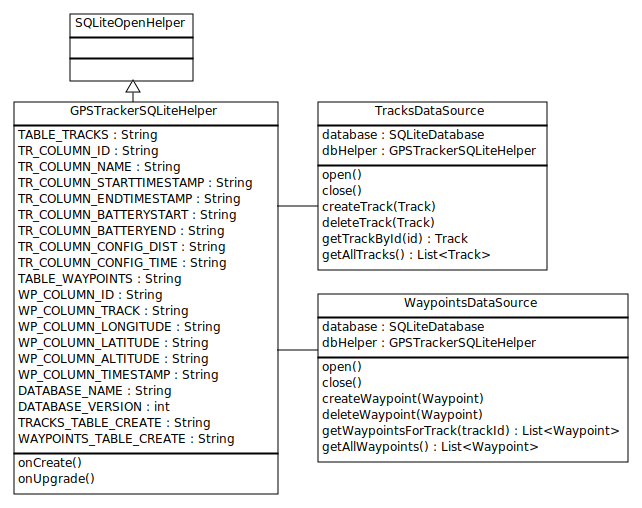
\includegraphics[width=0.6\textwidth]{images/classdiag_database.pdf}
  \caption[Klassendiagramm Datenbankanbindung]{Klassendiagramm Datenbankanbindung}
  \label{fig:classdiag_database}
\end{figure}

Zum Initialisieren der Datenbank und als Speicherort für die verwendeten Spalten- und Tabellennamen wurde der \lstinline$GPSTrackerSQLiteHelper$ verwendet. Dieser Helper ist von der Klasse SQLiteOpenHelper abgeleitet und überschreibt deren Methoden \lstinline$onCreate()$ und \lstinline$onUpdate()$. Die erstere wird aufgerufen, wenn die Datenbank noch nicht auf dem Device vorhanden ist. Die letztere wird aufgerufen, wenn die \lstinline$DATABASE_VERISON$ höher ist als diejenige, die beim erstellen der Datenbank auf dem Device aktuell war.

\lstinline$TracksDataSource$ und \lstinline$WaypointsDataSource$ bieten neben den $open()$ und $close()$ Methoden, welche eine Verbindung zur Datenbank herstellen beziehungsweise die Verbindung wieder trennen, ein Subset der üblichen CRUD \cite{crud} Methoden an, um die notwendigen Datenbankzugriffe auf eine möglichst einfache Art und Weise zu Verwalten. Im Listing \ref{lst:savetrackexample} ist an einem Beispiel ersichtlich, wie die \lstinline$TracksDataSource$ Klasse verwendet wird.

\begin{lstlisting}[caption={Beispiel: Track speichern}, label={lst:savetrackexample}]
TracksDataSource tds = new TracksDataSource(context);
tds.open(); //Connect database
tds.createTrack(track); //save track as new record 
tds.close(); //Close database connection
\end{lstlisting}

\subsection{Berechnung der Distanz}
\label{subsec:distance}
Die Distanz zwischen zwei Wegpunkten wird gemäss der Haversine Formel (Siehe Kapitel \ref{subsec:basicscalcdistance}) berechnet. Implementiert ist dies als Methode \lstinline$getDistanceTo(Waypoint)$ welche die Distanz zwischen dem aufrufenden und dem per Parameter übergebenen Waypoint, wie in Listing \ref{lst:distancecalc} ersichtlich, berechnet. Die Distanz eines ganzen Tracks entspricht der Summe der Distanzen zwischen allen Wegpunkten und ist in der Methode \lstinline$getDistance()$ der Track Klasse implementiert.

\begin{lstlisting}[caption={Distanzberechnung}, label={lst:distancecalc}]
private final static int R = 6371;
public double getDistanceTo(Waypoint other){
	double loThis = Math.toRadians(this.getLongitude());
	double laThis = Math.toRadians(this.getLatitude());
	double loOther = Math.toRadians(other.getLongitude());
	double laOther = Math.toRadians(other.getLatitude());
	
	double deltaLa = laThis-laOther;
	double deltaLo = loThis-loOther;
	
	double a = Math.pow(Math.sin(deltaLa/2), 2) + Math.cos(laThis) * Math.cos(laOther) * Math.pow(Math.sin(deltaLo/2), 2);
	double c = 2 * Math.atan2(Math.sqrt(a), Math.sqrt(1-a));
	return = R * c;
}
\end{lstlisting}

\subsection{Berechnung der Höhendifferenz}
\label{subsec:heightdifference}
Die Berechnung der Höhendifferenz (Listing \ref{lst:heightDifference}) hat drei Verschiedene Modi. Der Grund dafür lässt sich am besten an einem Beispiel erklären: Wenn man mit dem Velo von Göschenen (Rund 1100 m.ü.M.) auf den Gotthard Pass (rund 2100 m.ü.M) und danach weiter nach Airolo (rund 1175 m.ü.M) fährt, ist die Gesamthöhendifferenz 75 Meter. Abhängig von der körperlichen Verfassung wird der Velofahrer die 1000m, die er hoch gestrampelt ist, trotzdem in den Beinen spüren und entsprechend möchte er eine solche Angabe auch in einem GPS Tracker angezeigt bekommen. Basierend auf dieser Anforderung wurden die folgenden drei Modi entwickelt:

\begin{itemize}
\item positive: Die Summe aller Teilstrecken-Höhendifferenzen die positiv sind. (Im Gotthard Beispiel wären dies die ca. 1000m Bergauf)
\item negative: Die Summe aller Teilstrecken-Höhendifferenzen die negativ sind. (Im Gotthard Beispiel wären dies die ca. 925m Bergab)
\item total: Die Summe aller Teilstrecken-Höhendifferenzen. (Im Gotthard Beispiel ca. 75m)
\end{itemize}

\begin{lstlisting}[caption={Berechnung der Höhendifferenz}, label={lst:heightDifference}]
public double getHeightDifference(String mode) {
	if (waypoints.size() == 0 || waypoints.size() == 1) { //Cannot calculate height difference without waypoints
		return 0;
	} else {
		double sum = 0;
		for (int i = 1; i <= waypoints.size() - 1; i++) {
			double div = waypoints.get(i).getAltitude() - waypoints.get(i - 1).getAltitude();
			switch (mode) {
				case "positive": //only count positive height difference
					sum += div > 0 ? div : 0; break;
				case "negative": //only count negative height difference
					sum += div < 0 ? (-1) * div : 0; break;
				case "total": //count everything
					sum += div; break;
			}
		}
		return sum;
	}
}
\end{lstlisting}


\subsection{Akkumessung}
\label{subsec:battery}
Das auslesen der Batteriezustandes ist in der Privaten Methode \lstinline$getBatteryStatus$ des Tracks mithilfe des \lstinline$Intent.ACTION_BATTERY_CHANGED$ implementiert. Die Mtehode liest den Zustand der Batterie aus und gibt diesen als \lstinline$double$ zwischen 0 und 1 zurück. Mithilfe des Intents können sowohl \lstinline$level$ (Integer zwischen 0 und einem gerätespezifischen Maximum) als auch \lstinline$scale$ (Integer der dem gerätespezifischen Maximum entspricht) ausgelesen werden. Eine geräteunabhängige Angabe zwischen 0 und 1 berechnet sich daraus wie folgt: $batteryStatus=\frac{level}{scale}$ \cite{batterystatus}
\begin{lstlisting}[caption={Auslesen des Batterystatus}, label={lst:batterystatus}]
private double getBatteryStatus(Context context) {
	IntentFilter ifilter = new IntentFilter(Intent.ACTION_BATTERY_CHANGED);
	Intent batteryStatus = context.registerReceiver(null, ifilter);
	int level = batteryStatus.getIntExtra(BatteryManager.EXTRA_LEVEL, -1);
	int scale = batteryStatus.getIntExtra(BatteryManager.EXTRA_SCALE, -1);
	double batteryPct = level / (double) scale;
	return batteryPct;
}
\end{lstlisting}

\subsection{Android Frontend}
Das Android Frontend ist sehr einfach gestrickt. Es besteht aus drei Activities: Der \lstinline$SettingsActivity$, welche verwendet wird um die GPS-Tracking Parameter zu konfigurieren, der \lstinline$TrackListActivity$ welche die Track Liste anzeigt und der \lstinline$TrackDetailActivity$ - die Detailansicht für die einzelnen Tracks. Sowohl die TrackList als auch das TrackDetail Sheet wurden in Fragments (\lstinline$TrackListFragment$ und \lstinline$TrackDetailFragment$) so implementiert, dass auf einem Tablet nur eine Activity benötigt würde. Auf der linken Seite würde auf einem Tablet die Liste angezeigt und im Zentrum die jeweiligen Detail-Sheets.

\begin{figure}[h]
  \centering
  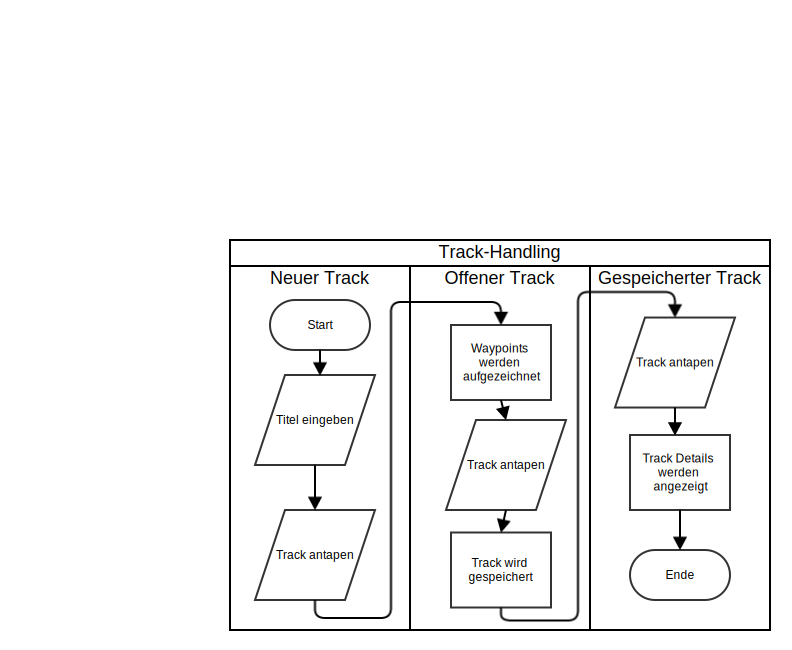
\includegraphics[width=0.8\textwidth]{images/trackworkflow.pdf}
  \caption[Track Lifecycle]{Track Lifecycle}
  \label{fig:tracklifecycle}
\end{figure}

Die Benutzerschnittstelle zum Erstellen von Tracks und zum Starten beziehungsweise Beenden des Trackings wurde so einfach wie möglich gehalten. In der Abbildung \ref{fig:tracklifecycle} ist in einem Flowchart der Track Lifecycle ersichtlich. Zum Erstellen eines Tracks, klickt der Benutzer aus der \lstinline$TrackList$ den Add Track Button. Nach dem Anklicken dieses Buttons wird der Benutzer nach einem Namen für den Track gefragt. Wenn er diesen eingibt und mit Ok bestätigt ist der Track als neuer Track in der Liste ersichtlich. Neue Tracks sind durch ein Play Symbol markiert. Wenn ein neuer Track angeklickt wird, beginnt der Trackingvorgang. Erneutes Anklicken beendet diesen und schreibt den Track in die Datenbank. Wenn gespeicherte Tracks angeklickt werden, öffnet sich das Detail-Sheet auf welchem verschiedene Informationen zum Track angezeigt werden.

\subsection{GPX Export}
\begin{figure}[h]
  \centering
  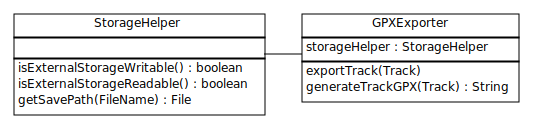
\includegraphics[width=0.6\textwidth]{images/classdiag_exporter.pdf}
  \caption[Klassendiagramm GPX Export]{Klassendiagramm GPX Export}
  \label{fig:gpxclassdiag}
\end{figure}

Das Exportieren von Tracks ins GPX Format wurde in der Klasse \lstinline$GPXExporter$ umgesetzt. Die Klasse bietet die zwei Methoden \lstinline$generateTrackGPX$ und \lstinline$exportTrack$ an. Die erstere nimmt einen Track entgegen und generiert daraus einen GPX XML String nach Spezifikation \cite{gpx}. Die letztere nimmt einen Track entgegen, findet mithilfe der entsrechenden Helper Klasse einen geeigneten Dateinamen auf Basis des Tracknamens, generiert das GPX XML mithilfe der \lstinline$generateTrackGPX$ Methode und schreibt dieses in das entsprechende File. Die Files werden im \lstinline$getExternalFilesDir(Environment.DIRECTORY_DOCUMENTS)$ \cite{savingfiles} abgelegt. Auf dieses Verzeichnis kann von einem PC aus zugegriffen werden. Wo genau es liegt, hängt vom verwendeten Gerät ab. 

Um Sicherzustellen, dass das externe Directory beschreibbar ist, wurde im Helper die Methode \lstinline$isExternalStorageWritable()$ implementiert, welche wie folgt prüft, ob das Verzeichnis beschreibbar ist:

\begin{lstlisting}[caption={Die isExternalStorageWritable Methode}, label={lst:isexternalstoragewriteable}]
public boolean isExternalStorageWritable() {
    String state = Environment.getExternalStorageState();
    if (Environment.MEDIA_MOUNTED.equals(state)) {
        return true;
    }
    return false;
}
\end{lstlisting}